\documentclass{article}
\usepackage{titlesec}

\usepackage[citestyle=authortitle-terse,backend=bibtex]{biblatex}
\addbibresource{bibliography.bib}

\setcounter{secnumdepth}{0}
\usepackage{sectsty}
\sectionfont{\fontsize{17}{20}\selectfont}

\usepackage[left=4cm, right=4cm]{geometry}
\usepackage{palatino,eulervm,dutchcal,xcolor}%fonts
\usepackage{graphicx,subcaption,float}
\usepackage{enumitem,parskip,multicol}
\usepackage{amsthm,amssymb,amsmath,mathtools,thmtools}
\usepackage{tikz,tikz-cd}
\usetikzlibrary{%
	matrix,%
	calc,%
	arrows,%
	shapes,
	decorations.markings,backgrounds,calc,intersections}
\tikzcdset{scale cd/.style={every label/.append style={scale=#1},
		cells={nodes={scale=#1}}}}
\usepackage[bookmarks,bookmarksopen,bookmarksdepth=3]{hyperref}
\hypersetup{%colores
	colorlinks=true,
	urlcolor=blue,
	linkcolor=magenta,
	citecolor=blue,
	filecolor=blue,
	urlbordercolor=white,
	linkbordercolor=white,
	citebordercolor=white,
	filebordercolor=white}
\usepackage{cleveref}
\Crefname{exercise}{Exercise}{Exercises}

\newcommand{\fakesection}[1]{%
	\par\refstepcounter{section}% Increase section counter
	\sectionmark{#1}% Add section mark (header)
	\addcontentsline{toc}{section}{\protect\numberline{\thesection}#1}% Add section to ToC
	% Add more content here, if needed.
}

\makeatletter %Hide section number
\def\@seccntformat#1{%
	\expandafter\ifx\csname c@#1\endcsname\c@section\else
	\csname the#1\endcsname\quad
	\fi}
\makeatother

\definecolor{blue-violet}{rgb}{0.54, 0.17, 0.89}
\definecolor{azure}{rgb}{0.0, 0.5, 1.0}
\definecolor{green(ncs)}{rgb}{0.0, 0.62, 0.42}
\definecolor{forestgreen}{rgb}{0.13, 0.55, 0.13}
\definecolor{limegreen}{rgb}{0.2, 0.8, 0.2}
\definecolor{palatinateblue}{rgb}{0.15, 0.23, 0.89}
\definecolor{trueblue}{rgb}{0.0, 0.45, 0.81}
\definecolor{goldenyellow}{rgb}{1.0, 0.87, 0.0}
\definecolor{fashionfuchsia}{rgb}{0.96, 0.0, 0.63}
\definecolor{brightcerulean}{rgb}{0.11, 0.67, 0.84}
\definecolor{jonquil}{rgb}{0.98, 0.85, 0.37}
\definecolor{lavendermagenta}{rgb}{0.93, 0.51, 0.93}
\definecolor{peru}{rgb}{0.8, 0.52, 0.25}
\definecolor{persimmon}{rgb}{0.93, 0.35, 0.0}
\definecolor{persianred}{rgb}{0.8, 0.2, 0.2}
\definecolor{persianblue}{rgb}{0.11, 0.22, 0.73}
\definecolor{persiangreen}{rgb}{0.0, 0.65, 0.58}
\definecolor{persianyellow}{rgb}{0.9, 0.89, 0.0}

\declaretheoremstyle[headfont=\color{trueblue}\normalfont\bfseries,]{colored1}
\declaretheoremstyle[headfont=\color{forestgreen}\normalfont\bfseries,]{colored2}
\declaretheoremstyle[headfont=\color{peru}\normalfont\bfseries,]{colored3}
\declaretheoremstyle[headfont=\color{persiangreen}\normalfont\bfseries,]{colored4}
\declaretheoremstyle[headfont=\color{brightcerulean}\normalfont\bfseries,]{colored5}
\declaretheoremstyle[headfont=\color{lavendermagenta}\normalfont\bfseries,]{colored6}
\declaretheoremstyle[headfont=\color{blue-violet}\normalfont\bfseries,]{colored7}
\declaretheoremstyle[headfont=\color{green(ncs)}\normalfont\bfseries,]{colored8}
\declaretheoremstyle[headfont=\color{peru}\normalfont\bfseries,]{colored9}
\declaretheoremstyle[headfont=\color{persiangreen}\normalfont\bfseries,]{colored10}
\declaretheoremstyle[headfont=\color{red}\normalfont\bfseries,]{colored11}

\declaretheorem[style=colored1,numberwithin=section,name=Theorem]{thm}
\declaretheorem[style=colored2,numberwithin=section,numberlike=thm,name=Proposition]{prop}
\declaretheorem[style=colored3,numberwithin=section,numberlike=thm,name=Lemma]{lemma}
\declaretheorem[style=colored4,numberwithin=section,numberlike=thm,name=Corollary]{coro}
\declaretheorem[style=colored5,numbered=no,name=Example]{example}
\declaretheorem[style=colored5,numbered=no,name=Examples]{exemplos}
\declaretheorem[style=colored7,numberwithin=section,name=Exercise]{exercise}
\declaretheorem[style=colored9,numbered=no,name=Remark]{remark}
\declaretheorem[style=colored9,numbered=no,name=Claim]{claim}
\declaretheorem[style=colored8,numbered=no,name=Definition]{defn}
\declaretheorem[style=colored11,numbered=no,name=Question]{question}

\newcommand{\R}{\mathbb{R}}
\newcommand{\Z}{\mathbb{Z}}
\newcommand{\N}{\mathbb{N}}
\newcommand{\C}{\mathbb{C}}
\newcommand{\Q}{\mathbb{Q}}
\newcommand{\D}{\mathbb{D}}
\newcommand{\T}{\mathbb{T}}
\renewcommand{\P}{\mathbb{P}}
\renewcommand{\H}{\mathbb{H}}
\newcommand{\Ac}{\mathcal{A}}
\newcommand{\Bc}{\mathcal{B}}
\newcommand{\Cc}{\mathcal{C}}
\newcommand{\Dc}{\mathcal{D}}
\newcommand{\Ec}{\mathcal{E}}
\newcommand{\Fc}{\mathcal{F}}
\newcommand{\Gc}{\mathcal{G}}
\newcommand{\Lc}{\mathcal{L}}
\newcommand{\Oc}{\mathcal{O}}
\newcommand{\Qc}{\mathcal{Q}}
\newcommand{\Sc}{\mathcal{S}}
\newcommand{\Wc}{\mathcal{W}}
\newcommand{\mf}{\mathfrak{m}}
\newcommand{\gf}{\mathfrak{g}}
\newcommand{\X}{\mathfrak{X}}
\newcommand{\hf}{\mathfrak{h}}
\newcommand{\glf}{\mathfrak{gl}}
\newcommand{\of}{\mathfrak{o}}

\renewcommand{\Im}{\operatorname{Im}}
\renewcommand{\O}{\operatorname{O}}
\renewcommand{\S}{\mathbb{S}}
\renewcommand{\T}{\mathbb{T}}
\DeclareMathOperator{\Lie}{\operatorname{Lie}}

\DeclareMathOperator{\img}{img}
\DeclareMathOperator{\Arg}{Arg}
\DeclareMathOperator{\End}{End}
\DeclareMathOperator{\I}{I}
\DeclareMathOperator{\id}{id}
\DeclareMathOperator{\Id}{Id}
\DeclareMathOperator{\Tr}{Tr}
\DeclareMathOperator{\Alt}{Alt}
\DeclareMathOperator{\sgn}{sgn}
\DeclareMathOperator{\supp}{supp}
\DeclareMathOperator{\Int}{Int}
\DeclareMathOperator{\Ob}{Ob}
\DeclareMathOperator{\Mor}{Mor}
\DeclareMathOperator{\Top}{Top}
\DeclareMathOperator{\CGWH}{CGWH}
\DeclareMathOperator{\Hom}{Hom}
\DeclareMathOperator{\Map}{Map}
\DeclareMathOperator{\Tot}{Tot}
\DeclareMathOperator{\Vect}{Vect}
\DeclareMathOperator{\VectBund}{VectBund}
\DeclareMathOperator{\Open}{Open}
\DeclareMathOperator{\Ring}{Ring}
\DeclareMathOperator{\Set}{Set}
\DeclareMathOperator{\GL}{GL}
\DeclareMathOperator{\SL}{SL}
\DeclareMathOperator{\SO}{SO}
\DeclareMathOperator{\U}{U}
\DeclareMathOperator{\SU}{SU}
\DeclareMathOperator{\Sp}{Sp}
\DeclareMathOperator{\M}{M}
\DeclareMathOperator{\Aut}{Aut}
\DeclareMathOperator{\PGL}{PGL}
\DeclareMathOperator{\PSL}{PSL}
\DeclareMathOperator{\St}{St}
\DeclareMathOperator{\Vol}{Vol}
\DeclareMathOperator{\Length}{Length}

\begin{document}
\begin{minipage}{\textwidth}
	\begin{minipage}{.5\textwidth}
		Complex Manifolds in Dimension 1\\
	\end{minipage}%
	\begin{minipage}{.5\textwidth}
		\raggedleft
		Daniel González Casanova Azuela\par
		{\small\href{https://github.com/dan-gc/riemann-surfaces}{github.com/dan-gc/riemann-surfaces}}
	\end{minipage}%
\end{minipage}\vspace{.2cm}\hrule
\section{Home Assignment 6: Isometries of $\H^2$}
\setcounter{section}{6}
\begin{defn}
	\textbf{\textit{Order}} of $A\in\GL(n)$ is the smallest positive integer such that $A^k=\Id$.
\end{defn}
\begin{exercise}
	Let $A$ be an element of finite order $k$ in $\GL(2,\Z)$. Prove that $k=2,3,4,6$.
\end{exercise}
\begin{proof}[Solution]
	(\textbf{From \href{https://math.stackexchange.com/questions/3759724/show-that-an-element-of-gl-2-mathbbz-has-order-1-2-3-4-6-or-infty}{StackExchange}.}) 
	First notice that $A$ is diagonalizable. This follows from the \href{https://en.wikipedia.org/wiki/Minimal_polynomial_(linear_algebra)#Applications}{fact} that a matrix is diagonalizable if and only if its minimal polynomial factors completely into distinct linear factors. The minimal polynomial $m_A$ of $A$ must divide any polynomial that annihilates $A$, so $m_A|X^k-1$. Also, $X^k-1$ factors into $k$ distinct linear factors given by the $k$-th roots of unity, and so does $m_A$.
	
	Let $\lambda_1$ and $\lambda_2$ be the eigenvalues of $A$, so that $\lambda_1^k=1$ and $\overline{\lambda}_2=\lambda_1$. Then there exists $\theta\in\R$ such that $\lambda_1=e^{i\theta}$ and $\lambda_2=e^{-i\theta}$. Since $A\in\GL(2,\Z)$ and the trace is invariant under change of coordinates, $\Tr A=\lambda_1+\lambda_2=2\cos\theta$ is an integer. Therefore, we have only 5 possibilities:
	\begin{align*}
		\cos\theta=1&\implies A^2=\Id\\
		\cos\theta=-1/2&\implies A^3=\Id\\
		\cos\theta=0&\implies A^4=\Id\\
		\cos\theta=1/2&\implies A^6=\Id\\
		\cos\theta=1&\implies A=\Id
	\end{align*}
\end{proof}

\begin{exercise}
	Let $A$ be an element of finite order $k$ in $\SL(3,\Z)$. Prove that $k=2,3,4,6$.
\end{exercise}
\begin{proof}[Solution]
	As in the former case, $A$ is diagonalizable. Again the trace of $A$ is an integer, and the eigenvalues satisfy $\overline{\lambda}_2=\lambda_1$ and $\lambda_3\in\R$. Moreover, its trace must be an integer. We have: \[\Tr(A)=\lambda_1+\lambda_2+\lambda_3=2\cos\theta+\lambda_3\in\Z,\]
	where $\theta$ is the real number such that $\lambda_1=e^{i\theta}$.
	
	We also know that the determinant of $A$, which is 1, must be the product of its eigenvalues:
	\[1=\det A=\lambda_1\lambda_2\lambda_3=|\lambda_1|^2\lambda_3=\lambda_3\]
	since, as in the previous exercise, $\lambda_1^k=1$. Finally, $2\cos\theta$ is again an integer and we conclude in analgous manner.
	
	%This means that again we must have $2\cos\theta\in\Z$ where $\theta$ is the real number such that $\lambda_1=e^{i\theta}$.
	%The product of its eigenvalues $\lambda_1$, $\lambda_2$ and $\lambda_3$ must be 1, and also each of them satisfies $\lambda^k_i=1$.
\end{proof}
\clearpage
\begin{exercise}
	Find an element of order $5$ in $\GL(4,\Z)$, or prove that it does not exist.
\end{exercise}
\begin{proof}[Solution]
	Suppose $A$ is an element of order 5 in $\GL(4,\Z)$. Once again, $A$ must be diagonalizable and its eigenvalues are two pairs of complex conjugates. In fact, since we want $A^5=\Id$, these eigenvalues must be the following two conjugate pairs of 5th roots of unity: 
	\begin{figure}[H]
		\centering
		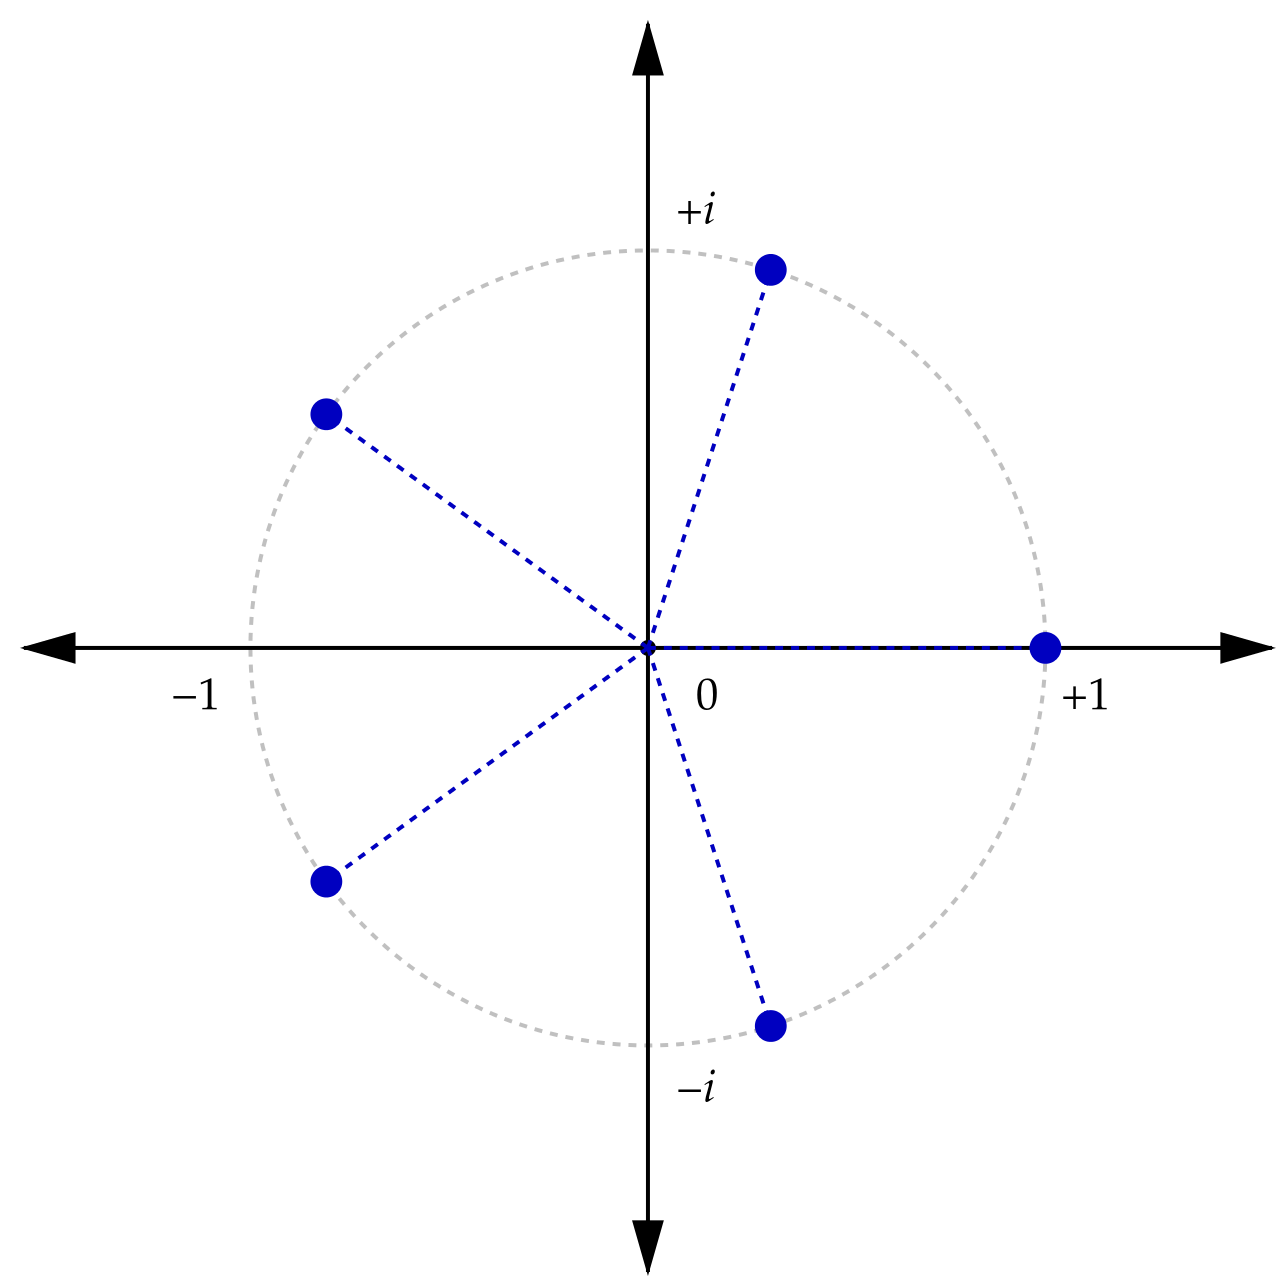
\includegraphics[width=0.5\linewidth]{../home-assignment5/5th-roots-of-unity}
		\label{fig:5th-roots-of-unity}
	\end{figure}	
	Up to a change of coordinates, if $\lambda_1=e^{i\theta}$ and $\lambda_2=e^{i\phi}$,
	\[\theta=\frac{2\pi\sqrt{-1}}{5}\qquad\text{and}\qquad\phi=\frac{4\pi\sqrt{-1}}{5}.\]
	
	However, the trace of $A$ must be an integer, that is
	\[\Tr A=2(\cos\theta+\cos\phi)\in\Z,\]
	which is not the case.
\end{proof}

\begin{remark}
	Let $V = \R^3$ be a vector space with quadratic form $q$ of signature $(1,2)$, $V^+:=\{v\in V|q(v)>0\}$, and $\P V^+$ its projectivisation. Then $\P V^+=\SO^+(1,2)/\SO(1)$, giving $\P V^+= \H^2$; this is one of the standard models of a hyperbolic plane. The \textbf{\textit{absolute}} is projectivization of the set of all isotropic lines; it is identified with the boundary of $\P V^+$ in $\P V$.
\end{remark}
\begin{defn}
	Let $\ell \subset V$ be a line, that is, a 1-dimensional subspace. The property $q(x,x)<0$ for a non-zero $x\in\ell$ is written as $q(\ell,\ell)<0$. A line $\ell$ with $q(\ell,\ell)<0$ is called \textbf{\textit{negative line}}, a line with $q(\ell,\ell) > 0$ is called \textbf{\textit{positive line}}.
\end{defn}
\begin{remark}
	Negative lines bijectively correspond to geodesics in $\P V^+ = \H^2$ (Lecture 8): an orthogonal complement to a negative line is a 2-dimensional plane $\ell^\perp$, its projectivization intersected with $\P V^+ = \H^2$ is a geodesic.
\end{remark}
\begin{exercise}
	 Let $\gamma_1$, $\gamma_2$ be geodesics on a hyperbolic plane, and $\ell_1$, $\ell_2$ the corresponding negative lines.
\end{exercise}
\begin{enumerate}[label*=\alph*.]
	\item Prove that $\ell_1$ is orthogonal to $\ell_2$ if and only if $\gamma_1$ is orthogonal to $\gamma_2$.
	\item Prove $\gamma_1$ intersects $\gamma_2$ if and only if the 2-plane $\langle\ell_1,\ell_2\rangle$ generated by $\ell_1$, $\ell_2$ has
	signature (0,2).
	
	\item Prove that $\gamma_1$ and $\gamma_2$ passes through the same point on the absolute if and only if
	the 2-plane generated by $\ell_1,\ell_2$ has degenerate scalar product.
	
\end{enumerate}

\begin{proof}[Attempt of solution]\leavevmode
\begin{enumerate}[label*=\alph*.]
	\item
	\begin{question}
		What is the definition of two hyperbolic geodesics being \textbf{\textit{orthogonal}}?
		
		Two planes in Euclidean space are naturally defined to be orthogonal if their normal vectors are orthogonal, but this would make the question tautological.
	\end{question}
	\begin{question}
		Can we actually have two orthogonal negative lines? 
		
		We find in \cite{vinberg} that
		\begin{quotation}
			{``A subspace $U\subseteq \R^{n,1}$ is said to be} \textit{elliptic} (respectively, \textit{parabolic}, \textit{hyperbolic}) if the restriction of the scalar product in $\R^{n,1}$ to $U$ is positive definite (respectively, positive semi-definite and degenerate, indefinite).
			\begin{figure}[H]
				\centering
				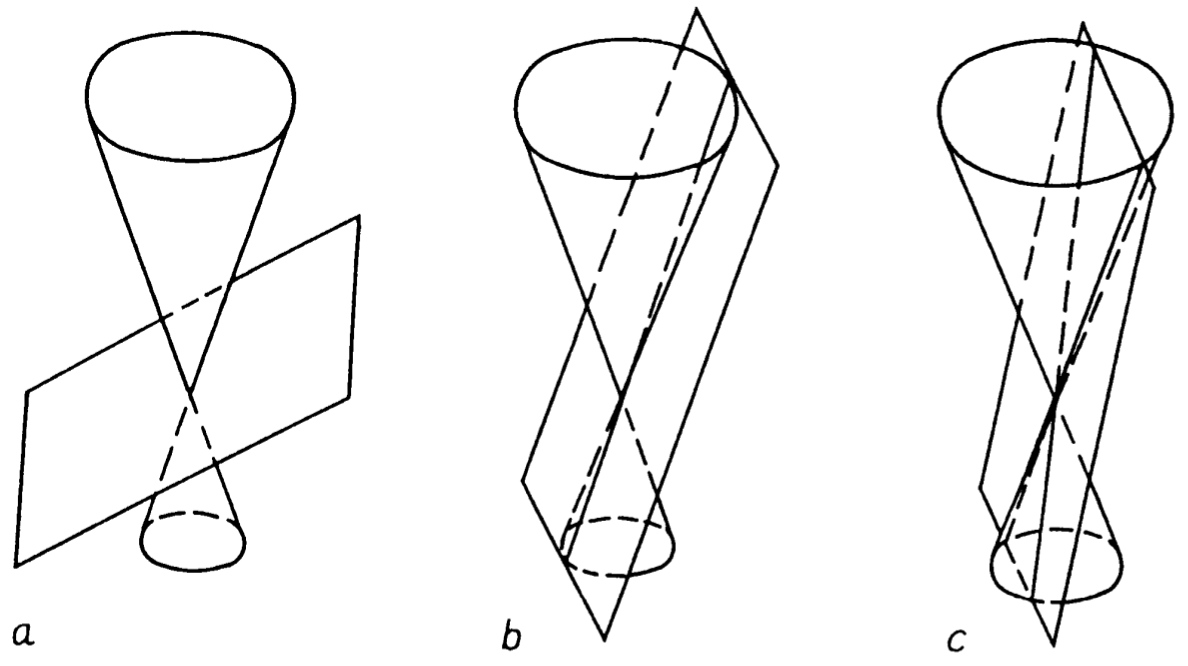
\includegraphics[width=0.7\linewidth]{../home-assignment5/vinberg}
				\caption*{Figure from \cite{vinberg}}
				\label{fig:vinberg}
			\end{figure}
			[...] The orthogonal complement $U^\perp$ to an elliptic (respectively, parabolic, hyperbolic) subspace $U$ is a hyperbolic (respectively, parabolic, elliptic) subspace."
		\end{quotation}
			which makes me think that given a negative (hyperbolic) line, any line orthogonal to it will be positive (elliptic), which is confusing.
		\end{question}
		
		\item 
			\begin{question}
				Two negative (hyperbolic) lines generate a plane that intersects the cone given by $q(x,x)=0$. (Such a plane is a hyperbolic subspace according to \cite{vinberg}.)
			
				I struggle to see how it could be possible that such a plane can have different signature depending wether the two geodesics intersect.
			\end{question}
			
			Two geodesics in $\P V^+$ do not intersect in $\H^2$ when their intersection is a negative point in $\P V$, that is, a point "inside" the cone. I have represented the situation when two geodesics do intersect:
		\begin{figure}[H]
			\centering
			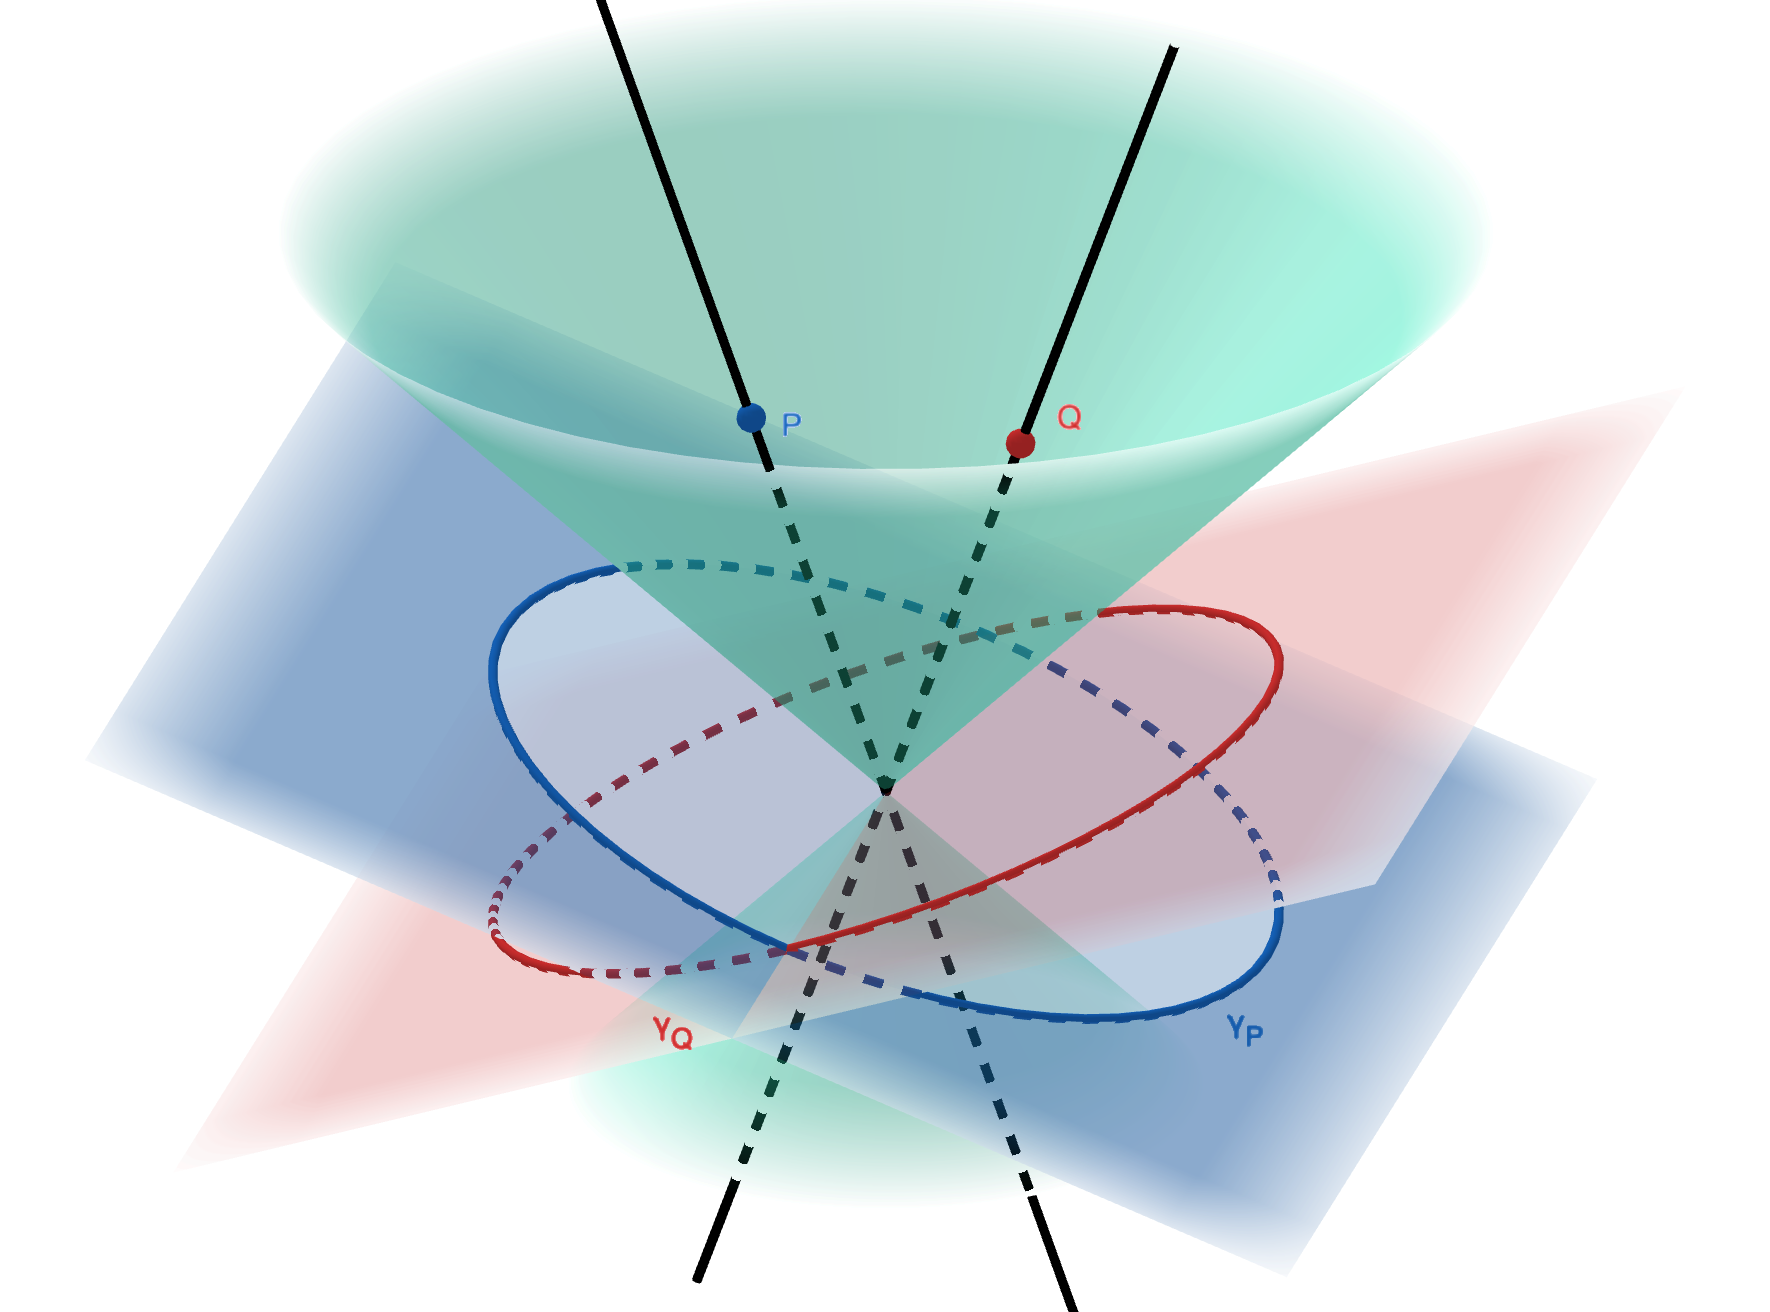
\includegraphics[width=1\linewidth]{geodesics}
			\caption*{Two negative lines determined by points $P$ and $Q$, their corresponding orthogonal planes and the intersection of the planes with a sphere centered about the origin. (See interactive figure  \href{https://www.geogebra.org/3d/h8kk2n7t}{online.})}
			\label{fig:geodesics1}
		\end{figure}
		
		\item This situation corresponds to the case when the planes corresponding to the geodesics are tangent to the cone. Scalar product in any of this planes is degenerate since each of them contains an isotropic line. The plane $\langle\ell_1,\ell_2\rangle$, a hyperbolic subspace, contains two isotropic lines and is also degenerate.
	\end{enumerate}
\end{proof}
\begin{remark}
	Review of definition of angle between geodesics is necessary to address d. and e. (and to correctly answer a. b. and c.).
\end{remark}
\iffalse
\begin{proof}[Attempt of solution]\leavevmode
	\begin{enumerate}[label*=\alph*.]
		\item It is clear that two euclidean-orthogonal lines will yield euclidean-orthogonal planes, as we can see in the following picture:
\iffalse		\begin{figure}[H]
			\centering
			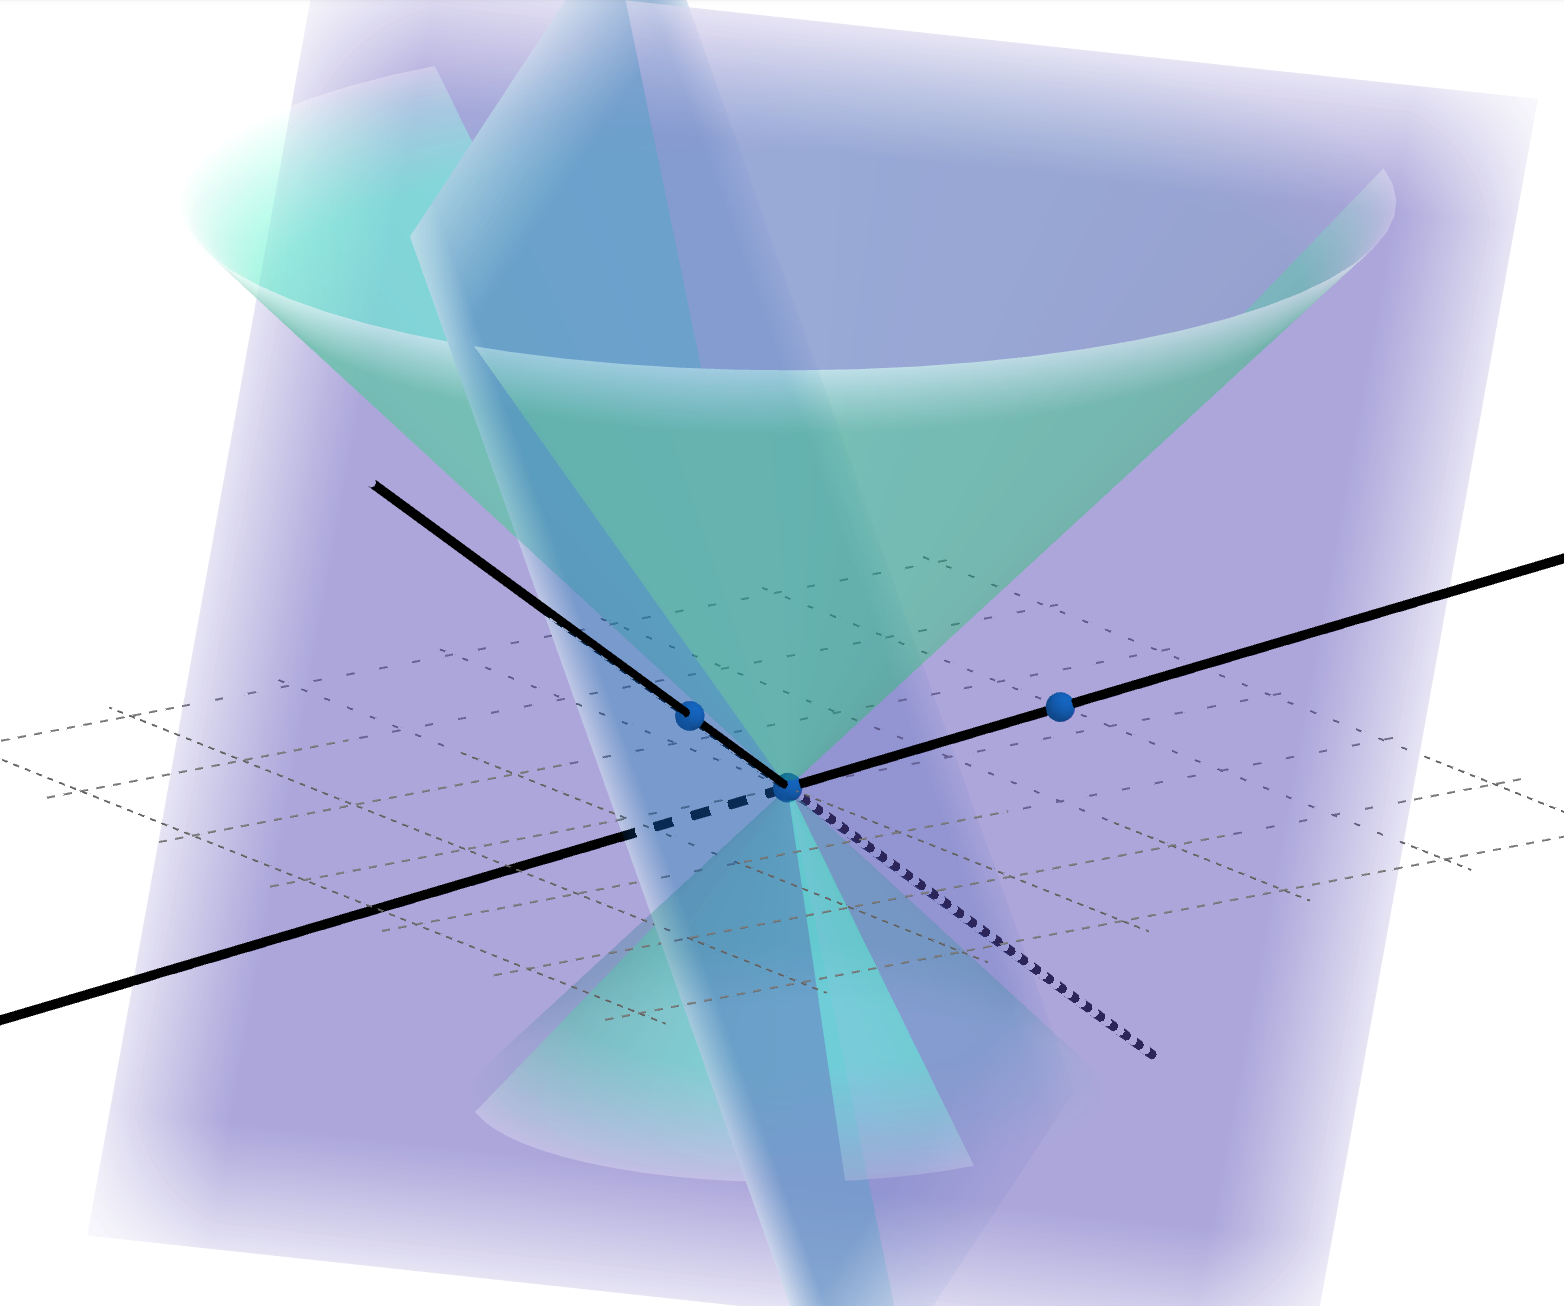
\includegraphics[width=0.7\linewidth]{../home-assignment5/lines1}
			\caption{Two orthogonal lines and their corresponding planes}
			\label{fig:lines1}
		\end{figure}\fi
		More formally, in the euclidean case we simply have that two lines are orthogonal if and only if their corresponding planes are orthogonal because $\ell_1\perp\ell_2\implies\ell_1\subset\ell_2^\perp$ and $\ell_2\subset\ell_1^\perp$ and 
		
		Whenever a plane $\Pi_1$ contains a line $\ell_2$ orthogonal to another plane $\Pi_2$, then $\Pi_1\perp\Pi_2$ by linearity of the dot product. Indeed any $v\in\Pi_1$ is of the form $v_2+v'$ with $v_2\in\ell_2$ so for any $w\in\Pi_2$ we have \[\langle v, w\rangle=\langle v_2+v',w\rangle=\langle v_2,w\rangle+\langle v',w\rangle=\langle v',w\rangle\]
		But also $\Pi_2$ contains a line $\ell_1$ orthogonal to $\Pi_1$, so $w=w_1+w'$ with $w_1\in\ell_1$ so
		\[\langle v',w\rangle=\langle v',w_1+w'\rangle=\langle v',w_1\rangle+\langle v',w'\rangle=\langle v',w'\rangle\]
		
		Now consider orthogonality with respect to $q$. 
		
		\begin{itemize}
			\item $\ell_1$ orthogonal to $\ell_2$ means that $q(x,y)=0$ for all $x\in\ell_1$ and all $y\in\ell_2$.
			\item $\gamma_1$ orthogonal to $\gamma_2$ means that $q(v,w)=0$ for all $v\in\ell_1^\perp$ and all $w\in\ell_2^\perp$.
		\end{itemize}
		$(\implies)$ $v\in\ell^\perp_1\iff q(x,v)=0\;\forall x\in\ell_1$, so that if we had $w\in\ell_1$, we would be done. But all we know is that $w\in\ell^\perp_2\iff q(y,w)=0\;\forall y\in\ell_2$.
		
		$(\impliedby)$ Let $x\in\ell_1$ and $y\in\ell_2$. Since 

		\item 
	\end{enumerate}
\end{proof}\fi

\begin{remark}
	Recall that $h \in \SO^+(1, 2)$ is called \textbf{\textit{hyperbolic}} if it has an eigenvalue $\alpha$ with $|\alpha| > 1$.
\end{remark}
\begin{exercise}
	Let $q$ be a quadratic form of signature $(1,2)$ on $\R^3$ with integer coefficients, $h \in \SO^+(1,2)$ a hyperbolic matrix with integer coefficients, and $P_h(t)$ its characteristic polynomial. Prove that $P_h(t)$ has precisely 1 rational root.
\end{exercise}
	No solution so far.
	I have asked this question on \href{https://math.stackexchange.com/questions/4911600/hyperbolic-isometry-must-have-precisely-one-rational-eigenvalue?noredirect=1#comment10486659_4911600}{StackExchange}.
\printbibliography
\end{document}